% Fachstudie NEXUS "Personen im Raum"
% $Id: pir.tex,v 1.12 2005/05/26 22:24:11 garbeam Exp $

\documentclass{article}
\usepackage[german]{babel} 
\usepackage[latin1]{inputenc}
\usepackage[T1]{fontenc}
\usepackage{fancyhdr}
\usepackage{times}
\usepackage[dvips]{graphicx}
\usepackage{url}

\begin{document}

\title{Fachstudie 'Personen im Raum'}
\author{Steffen Keul, Marcel Kilgus, Anselm Garbe\\
\small Universit�t Stuttgart, Institut f�r Informatik, Nexus Forschungsprojekt}

\maketitle
\thispagestyle{empty}

\begin{abstract}
In dieser Fachstudie wird die Bewegungserkennung von Personen auf
Bilddaten eines Raumes mithilfe verschiedener Algorithmen aus der
OpenSource Vektor-Grafik Bibliothek OpenCV\cite{opencv} untersucht.
Die Bilddaten werden durch eine handels�bliche Web-Kamera geliefert.
Die Ergebnisse der Bewegungserkennung werden in
Characteristic-Receiver-Operator Curves veranschaulicht. Abschlie�end
wird die Eignung der untersuchten Algorithmen bewertet.
\end{abstract}

%------------------------------------------------------------------------- 
\section{Einleitung}
Im Rahmen des Nexus Forschungsprojektes, das die Realisierung mobiler
kontext-bezogener Systeme in geeigneten Umgebungsmodellen untersucht,
stellt sich u.a. die Aufgabenstellung durch Bilderkennung von Objekten
spezielle kontext-bezogene Reaktionen in solchen Systeme zu realisieren.
Eine einfache Anwendung w�re beispielsweise die akustische Ausgabe einer
Meldung durch ein System, wenn die letzte Person bei ge�ffnetem
Fenster einen Raum verl��t, das Fenster zu schlie�en.
Um eine solche Anwendung realisieren zu k�nnen mu� zun�chst ein
geeigneter Weg zur Bilderkennung gefunden werden.


%------------------------------------------------------------------------- 
\section{Ziel}
Ziel dieser Fachstudie ist die Evaluierung der Eignung von folgenden
Bilderkennungs-Algorithmen aus der OpenCV\cite{opencv} Bibliothek:

\begin{itemize}
\item CalcOpticalFlowHS
\item CalcOpticalFlowLK
\item CalcOpticalFlowBM
\item CalcOpticalFlowPyrLK
\item SegmentMotion
\end{itemize}

Es werden Bilddaten eines Raumes einer handels�blichen Web-Kamera zur Untersuchung
verwendet. Ein Algorithmus, der zuverl�ssig Bewegungen auf
Bildsequenzen dieser Bilddaten erkennt, kann f�r Aussagen zur Erkennung
von Objekten in Betracht gezogen werden.
Personen sind keine starren Objekte und zeigen Ver�nderungen in Form von
Bewegungen zwischen einzelnen Bildern einer Bildsequenz auf.
Die Erkennung solcher Bewegungen kann zu einer Existenzaussage
von Personen im Bildausschnitt approximiert werden. Dar�ber stellt sich
die Frage, in wie weit sich solche Existenzaussagen zur Z�hlung von
Personen eignen und welche Bedingungen sich daran kn�pfen.

Neben diesen Bewertungen wird ein kleiner Vergleich auf vorhandene
technische Systeme zur Bewegungserkennung gegeben, die auf Bilderkennung
basieren, sowie ein zur untersuchten Vektor-Grafik-Bibliothek
alternatives Produkt.

% Vgl. OpenCV mit anderen Bibliotheken zB MontiVision Development Kit
% OpticalFlow Modul
% evtl. andere Prozesse

%------------------------------------------------------------------------- 
\section{Bilddaten}

Die verwendeten Bilddaten werden mit einer handels�blichen WebCam, Modell MOBOTIX M1
(\url{http://www.mobotix.com}), unter identischen Lichtbedingungen und
unver�ndertem Raumausschnitt erzeugt.
Die Kameraeinstellungen und Bildeigenschaften sind wie folgt festgelegt:

\begin{figure}[h]
    \begin{center}
        \begin{tabular}{l|l}
        \textbf{Format:} & JPEG\\ \hline
        \textbf{Kompression:} & Standard\\ \hline
        \textbf{Aufl�sung (Pixel):} & 640x480\\ \hline
        \textbf{Automatischer Lichtfilter:} & aus\\ \hline
        \textbf{Rauschenunterdr�ckung:} & aus\\ \hline
        \textbf{Hintergrundlicht (-10..10):} & 0\\
        \textbf{S�ttigung (-10..10):} & 0\\
        \textbf{Bildsch�rfe (-2..20):} & 0\\
        \end{tabular}
    {\small \caption{Kameraeinstellungen}}
    \end{center}
\end{figure}

Es werden zur Untersuchung jeweils eine Bildsequenz von 200 Bildern pro
Szenario erstellt.

%------------------------------------------------------------------------- 
\section{Szenarien}
Es werden zwei Szenarien untersucht:

\begin{itemize}
\item keine Person im Bild
\item bewegte Personen im Bild
\end{itemize}

Im ersten Szenario ist keine Person im Bildausschnitt aller 200
Bildsequenzen sichtbar. Im anderen Szenario sind teilweise keine Person
sichtbar, eine Person und mehrere Personen die sich bewegen.

%------------------------------------------------------------------------- 
\section{Algorithmen}

\subsection{CalcOpticalFlowHS}
Dieser Algorithmus berechnet den optischen Bewegungsfluss f�r alle Pixel
zwischen zwei Bildern nach dem Horn \& Schunk \cite{Horn81} Verfahren.

\subsection{CalcOpticalFlowLK}
Dieser Algorithmus berechnet den optischen Bewegungsfluss f�r alle Pixel
zwischen zwei Bildern nach dem Lucas \& Kanade \cite{Lucas81} Verfahren.

\subsection{CalcOpticalFlowBM}
Dieser Algorithmus berechnet den optischen Bewegungsfluss f�r
Segmente einer frei definierbaren Gr��e zwischen zwei Bildern.
Um so gr�ber die Segmente gew�hlt werden, desto performanter arbeitet der
Algorithmus.

\subsection{CalcOpticalFlowPyrLK}
Dieser Algorithmus \cite{Bouget00} basiert auf einer iterativen Version der optischen
Fluss-Pyramiden nach Lucas \& Kanade. Er berechnet den optischen
Bewegungsfluss auf einer Menge von Punkten zwischen zwei Bildern. Es
werden Bewegungen mit Sub-Pixel Genauigkeit gefunden.

\subsection{SegmentMotion}
Dieser Algorithmus sucht alle bewegten Segmente zwischen zwei Bildern
und vergibt f�r jede Bewegung in einer Segmentmaske Werte zwischen
$1..N$, je nach Bewegungsintensit�t.

\subsection{Eigene Implementierung}
Neben den genannten Algorithmen aus der Vektor-Grafik-Bibliothek
OpenCV\cite{opencv} wurde auch ein eigener Algorithmus entworfen und
untersucht, der unter einer einstellbaren Unsch�rfeschwelle
Differenzbilder zwischen zwei Bildern erzeugt. Wenn Differenzen
existieren, so werden diese als Bewegungsfelder auf dem Differenzbild
sichtbar.

%------------------------------------------------------------------------- 
\section{Receiver Operator Characteristic Curves}


\includegraphics[width=7cm,angle=270]{impl/motion-1-d1.log.ps}



\includegraphics[width=7cm,angle=270]{impl/motion-1-d10.log.ps}



\includegraphics[width=7cm,angle=270]{impl/motion-1-d10m001M1.log.ps}




\includegraphics[width=7cm,angle=270]{impl/motion-1-d10m001M3.log.ps}




\includegraphics[width=7cm,angle=270]{impl/motion-1-d1m001M1.log.ps}




\includegraphics[width=7cm,angle=270]{impl/motion-1-d1m001M3.log.ps}




\includegraphics[width=7cm,angle=270]{impl/motion-1-d2.log.ps}




\includegraphics[width=7cm,angle=270]{impl/motion-1-d2m001M1.log.ps}




\includegraphics[width=7cm,angle=270]{impl/motion-1-d2m001M3.log.ps}




\includegraphics[width=7cm,angle=270]{impl/motion-1-d3.log.ps}




\includegraphics[width=7cm,angle=270]{impl/motion-1-d3m001M1.log.ps}




\includegraphics[width=7cm,angle=270]{impl/motion-1-d3m001M3.log.ps}




\includegraphics[width=7cm,angle=270]{impl/motion-1-d5.log.ps}




\includegraphics[width=7cm,angle=270]{impl/motion-1-d5m001M1.log.ps}




\includegraphics[width=7cm,angle=270]{impl/motion-1-d5m001M3.log.ps}




\includegraphics[width=7cm,angle=270]{impl/motion-2-d1.log.ps}




\includegraphics[width=7cm,angle=270]{impl/motion-2-d10.log.ps}




\includegraphics[width=7cm,angle=270]{impl/motion-2-d10m001M1.log.ps}




\includegraphics[width=7cm,angle=270]{impl/motion-2-d10m001M3.log.ps}




\includegraphics[width=7cm,angle=270]{impl/motion-2-d1m001M1.log.ps}




\includegraphics[width=7cm,angle=270]{impl/motion-2-d1m001M3.log.ps}




\includegraphics[width=7cm,angle=270]{impl/motion-2-d2.log.ps}




\includegraphics[width=7cm,angle=270]{impl/motion-2-d2m001M1.log.ps}




\includegraphics[width=7cm,angle=270]{impl/motion-2-d2m001M3.log.ps}




\includegraphics[width=7cm,angle=270]{impl/motion-2-d3.log.ps}




\includegraphics[width=7cm,angle=270]{impl/motion-2-d3m001M1.log.ps}




\includegraphics[width=7cm,angle=270]{impl/motion-2-d3m001M3.log.ps}




\includegraphics[width=7cm,angle=270]{impl/motion-2-d5.log.ps}




\includegraphics[width=7cm,angle=270]{impl/motion-2-d5m001M1.log.ps}




\includegraphics[width=7cm,angle=270]{impl/motion-2-d5m001M3.log.ps}




\includegraphics[width=7cm,angle=270]{impl/pyramid-f1-1.log.ps}




\includegraphics[width=7cm,angle=270]{impl/pyramid-f1-2.log.ps}




\includegraphics[width=7cm,angle=270]{impl/pyramid-f2-1.log.ps}




\includegraphics[width=7cm,angle=270]{impl/pyramid-t05-f1-1.log.ps}




\includegraphics[width=7cm,angle=270]{impl/pyramid-t05-f1-2.log.ps}




\includegraphics[width=7cm,angle=270]{impl/pyramid-t05-f2-1.log.ps}




\includegraphics[width=7cm,angle=270]{impl/pyramid-t05-f2-2.log.ps}




\includegraphics[width=7cm,angle=270]{impl/pyramid-t100-f1-1.log.ps}




\includegraphics[width=7cm,angle=270]{impl/pyramid-t100-f1-2.log.ps}




\includegraphics[width=7cm,angle=270]{impl/pyramid-t100-f2-1.log.ps}




\includegraphics[width=7cm,angle=270]{impl/pyramid-t100-f2-2.log.ps}




\includegraphics[width=7cm,angle=270]{impl/pyramid-t50-f1-1.log.ps}




\includegraphics[width=7cm,angle=270]{impl/pyramid-t50-f1-2.log.ps}




\includegraphics[width=7cm,angle=270]{impl/pyramid-t50-f2-1.log.ps}




\includegraphics[width=7cm,angle=270]{impl/pyramid-t50-f2-2.log.ps}




\includegraphics[width=7cm,angle=270]{impl/test-1.log.ps}




\includegraphics[width=7cm,angle=270]{impl/test-2.log.ps}




%------------------------------------------------------------------------- 
\section{Empfehlung}
Im Rahmen dieser Fachstudie empfehlen wir die optische Flusserkennung
nach \cite{KIL05}, die auch im Source Code im Anhang vorliegt.

\begin{thebibliography}{99}
\bibitem{opencv} http://opencvlibrary.sf.net
\bibitem{KIL05} Marcel Kilgus, Optische Flusserkennung mit 15 LOC, 2005.
\bibitem{Horn81} Berthold K. P. Horn und Brian G. Schunck. Determining
Optical Flow. Artificial Intelligence, 17, pp. 185-203, 1981.
\bibitem{Lucas81} Lucas, B. und Kanade, T. An Iterative Image
Registration Technique with an Application to Stereo Vision, Proc. of
7th International Joint Conference on Artificial Intelligence (IJCAI),
pp. 674-679.
\bibitem{Bouget00} Jean-Yves Bouguet. Pyramidal Implementation of the
Lucas Kanade Feature Tracker.
\end{thebibliography}

\end{document}
